\section{Ray Tracing} \label{sec:ray-tracing}

El \textit{Ray Tracing} es un algoritmo de renderizado en el que una imagen se
crea identificando los objetos que contribuyen a cada pixel (\textit{image-order
  rendering}). Dada una escena con objetos tridimensionales, se puede obtener una
imagen de la misma lanzando rayos desde un origen (cámara) hacia una ventana, y
trazando la trayectoria de los mismos para ver sobre qué objetos / materiales
incidió (Figura \ref{fig:rt-camera-throwing-rays-into-scene}).

\begin{figure}
  \centering
  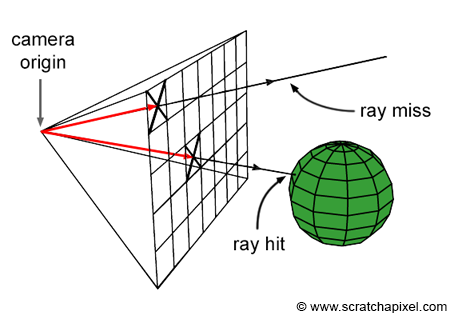
\includegraphics[width=.7\textwidth]{imgs/rt-camera-throwing-rays-into-scene.png}
  \caption{Cámara lanzando rayos por una ventana hacia una escena}
  \label{fig:rt-camera-throwing-rays-into-scene}
\end{figure}

La imagen final es el resultado de muchas variables:

\begin{itemize}
  \item Cámara: posición, dirección, inclinación, apertura de la lente,
        distancia de foco.
  \item Objetos: ubicación, tamaños, formas, etc.
  \item Materiales (de cada objeto): tipos (lambertiano, metálico, etc),
        color, reflexión, refracción, etc.
  \item Archivo de salida: Dimensiones, \textit{spp}, \textit{max depth}.
\end{itemize}

A continuación explicaremos como cada uno influye en la imagen final.

\subsection{Cámara} \label{ssec:rt-camera}

La cámara es una parte fundamental del ray tracing. Sin objetos, obtenemos una
imagen vacía, pero sin cámara, simplemente no hay imagen.

Para generar la imagen final, se utiliza la \textbf{posición} de la cámara como
el origen de los rayos, y la \textbf{dirección} en la que apunta para establecer
donde se encuentra el plano de foco, donde se construye la ventana que
finalmente corresponde con la imagen. También es necesario conocer la
\textbf{dirección arriba}: si la cámara fuese la de un celular, la dirección
arriba estaría dada por la inclinación.

Por otro lado, el \textbf{field of view} establece las dimensiones de la
ventana, mientras que la \textbf{apertura} y la \textbf{distancia de foco}
establecen el \textit{nivel de enfoque} de la imagen. Esto se logra usando como
verdadero origen de los rayos un disco de diámetro \textit{aperture}, a
distancia \textit{focus\_dist} de la ventana (ver figura
\ref{fig:rt-camera-plano-foco}).

\begin{figure}[H]
  \centering
  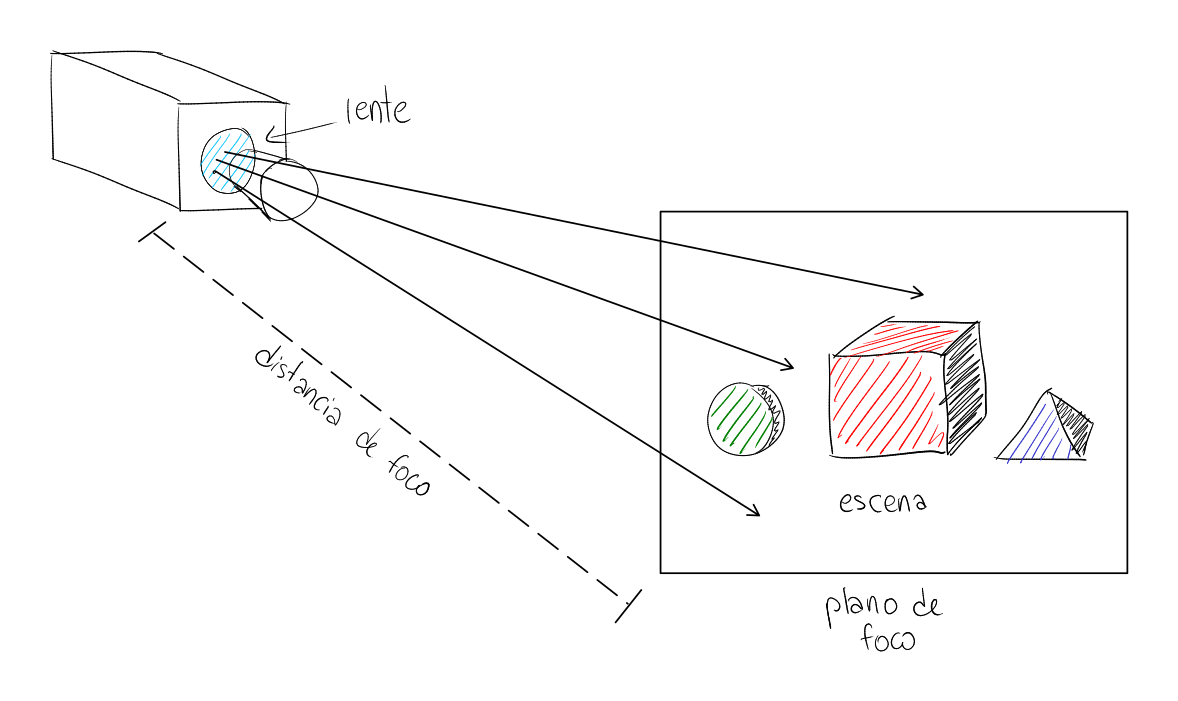
\includegraphics[width=.7\textwidth]{imgs/rt-camera-rays-through-lens.png}
  \caption{Lente y plano de foco}
  \label{fig:rt-camera-plano-foco}
\end{figure}

Los rayos se lanzarán desde un punto aleatorio de la lente, hacia distintos
puntos en el plano de foco (dependiendo del pixel que se esté calculando).
Mientras más chico sea el diámetro de la lente, y más cerca esté el plano de
foco del objetivo, más nítida será la imagen. Por el contrario, si la lente es
muy grande, o el plano de foco se encuentra lejos del objetivo, la imagen se
verá más borrosa.

Cuando un rayo colisiona con un objeto, queda determinado un nuevo rayo saliente
del punto de intersección, siempre y cuando no se supere el \texttt{max\_depth}.
El nuevo rayo puede generarse por reflexión o por refracción (dependiendo del
material del objeto), y su dirección también depende de la forma del objeto.

Por cada pixel de la imagen, se envían tantos rayos como lo indique el
\texttt{spp}. Los rayos ``rebotan'' por la escena hasta que se supere el
\texttt{max\_depth}, se acumula el color de todos los objetos con los que el
rayo colisionó en su trayectoria, y finalmente el color de todas las colisiones
se promedia para calcular el color final del pixel.

\subsection{Objetos}

Los objetos son cuerpos del espacio tridimensional que pueden colisionar con los
rayos y en consecuencia, modificar la trayectoria de los mismos y finalmente la
imagen. Dependiendo del material de su superficie, estos pueden reflejar o
refractar los rayos, y cambiar el color de cada pixel. En este trabajo se
implementaron 5 tipos objetos:

\begin{itemize}
  \item Esferas
  \item Planos
  \item Cubos
  \item Triángulos
  \item KDTree
\end{itemize}

Cada objeto es definido por una función que indica si un rayo colisiona o no con
el mismo (\texttt{hit}). Además, esta función retorna (en caso de que haya
colisión) detalles de como se dio la misma: el punto de intersección, la normal
de la superficie en ese punto, el material del objeto, etc.

Por ejemplo, la función \texttt{hit} de un plano devuelve verdadero si el rayo
\textbf{no} es paralelo al plano (suponiendo que el rayo y el plano no se
superponen). Por otro lado, para una esfera la función devuelve verdadero si el
rayo ``pasa'' lo suficientemente cerca del origen (radio de la esfera).

Formalmente, representaremos a un rayo como un par $\left\langle P, D
  \right\rangle$, donde $P$ es el punto de origen y $D$ es la dirección. De esta
forma, podemos describir cada punto del rayo $R(t) = P + tD$. La función
\texttt{hit} de un objeto recibirá como parámetros:

\begin{itemize}
  \item El objeto, para saber sus coordenadas y dimensiones
  \item El rayo
  \item $t_{min}$ y $t_{max}$: el rango de valores de $t$ (del rayo) a
        considerar. Por ejemplo, no consideramos colisiones con $t < 0$ porque
        se encuentran detrás de la cámara y no aparecen en la imagen final
\end{itemize}

Y retornará dos valores:

\begin{itemize}
  \item Un booleano, para indicar si hay intersección o no
  \item Un diccionario con los datos de la colisión, si corresponde
\end{itemize}

Como vimos, la implementación de cada función \texttt{hit} puede ser muy
diferente dependiendo de la forma y las propiedades de cada objeto, así que
exploraremos cada uno por separado.

\subsubsection{Plano}

Un plano está dado por un origen $O$ y una normal $N$. Para decidir si un rayo
$R(t)$ interseca con el plano, bastará con ver que no sean paralelos. El punto
de intersección (en particular, el parámetro $t$ del rayo) se puede despejar de
la ecuación del plano, si planteamos la igualdad en el punto de intersección:

\begin{align*}
  ((P + tD) - O) \cdot N         & = 0                                 \\
  (tD \cdot N) + (P - O) \cdot N & = 0                                 \\
  t(D \cdot N)                   & = (O - P) \cdot N                   \\
  t                              & = \frac{(O - P) \cdot N}{D \cdot N} \\
\end{align*}

\begin{algorithm}[H]
  \begin{algorithmic}[1]
    \Function{PlaneHit}{$Plane, Ray, t_{min}, t_{max}$}{$\rightarrow (hit, record)$}
    \State $O, N \gets Plane$ \Comment{Descomponemos en origen y normal}
    \State $P, D \gets Ray$ \Comment{Descomponemos en origen y dirección}
    \If {$N \perp D$} \Comment{Rayo y plano son paralelos}
    \State \Return (False, NIL)
    \EndIf
    \State $t \gets ((O - P) \cdot N)/(D \cdot N)$

    \If {$\lnot (t_{min} \le t \le t_{max})$} \Comment{Punto fuera del rango permitido}
    \State \Return (False, NIL)
    \EndIf

    \State $record \gets$ ($t$, $N$, \dots) \Comment{Datos de la intersección}
    \State \Return (True, $record$)
    \EndFunction
  \end{algorithmic}
  \caption{Algoritmo \textit{hit} para planos}
  \label{alg:plane-hit}
\end{algorithm}

El algoritmo \ref{alg:plane-hit} refleja este procedimiento. Devuelve un par
$(hit, record)$ donde $hit$ es un booleano que indica si hubo intersección, y
$record$ contiene los datos de la misma (como la ``distancia'' desde el origen
del rayo $t$, o la normal del plano de intersección $N$), o \texttt{NIL} si no
hubo intersección.

\subsubsection{Esferas}

Para representar una esfera definimos $C = (C_x, C_y, C_z)$ al centro de la
misma, y $r$ al radio. La ecuación de los puntos $Q=(x, y, z)$ de la superficie
de la misma está dada por:

\begin{align*}
  (x - C_x)^2 + (y - C_y)^2 + (z - C_z)^2 & = r^2 \\
  (Q - C) \cdot (Q - C) = r^2
\end{align*}

Como $Q = R(t) = P + tD$ en la intersección, podemos reemplazarlo en la ecuación
y obtener una ecuación cuadrática en $t$.

\begin{align*}
  (P + tD - C) \cdot (P + tD - C)                                  & = r^2 \\
  D t^2 \cdot D + 2D \cdot (P - C) t + (P - C) \cdot (P - C) - r^2 & = 0
  \label{eq:cuad-esfera}
\end{align*}

Esta función puede tener 0, 1 o 2 raíces, dependiendo de si el rayo interseca o
no con la esfera, y en cuantos puntos lo hace. Si la función no tiene raíces, no
existe $t$ que satisfaga la ecuación de la esfera, y, por lo tanto, no hay
intersección. Si la función tiene 1 raíz, el rayo interseca a la esfera en
\textbf{un} único punto, y es tangente a la superficie de la misma. Por otro
lado, si la función tiene 2 raíces, el rayo atraviesa la esfera y la interseca
en 2 puntos, uno de entrada y uno de salida.

Para determinar si existe intersección, podemos calcular el discriminante y ver
si es positivo (hay intersección) o no.

\begin{algorithm}
  \begin{algorithmic}[1]
    \Function{SphereHit}{$Sphere, Ray, t_{min}, t_{max}$}{$\rightarrow (hit, record)$}
    \State $C, r \gets Sphere$ \Comment{Descomponemos en centro y radio}
    \State $P, D \gets Ray$ \Comment{Descomponemos en origen y dirección}
    \State $a \gets D \cdot D$
    \State $b \gets 2D \cdot (P - C)$
    \State $c \gets (P - C) \cdot (P - C) - r^2$
    \State $disc \gets b^2 - 4ac$

    \If {$disc < 0$}
    \State \Return (False, \texttt{NIL})
    \EndIf

    \State $t \gets (-b - \sqrt{disc} / 2a)$
    \If {$t < t_{min} \lor t_{max} < t$}
    \State $t \gets (-b + \sqrt{disc} / 2a)$
    \If {$t < t_{min} \lor t_{max} < t$}
    \State \Return (False, \texttt{NIL})
    \EndIf
    \EndIf

    \State $N \gets P + tD - C$ \Comment{Normal al plano de la intersección}
    \State $record \gets$ ($t$, $N$, \dots) \Comment{Datos de la intersección}
    \State \Return (True, $record$)
    \EndFunction
  \end{algorithmic}
  \caption{Algoritmo \textit{hit} para esferas}
  \label{alg:sphere-hit}
\end{algorithm}

\subsubsection{Cubos}

La forma más directa de implementar cubos es utilizando planos para representar
cada cara. Para simplificar la implementación, solo representaremos cubos
alineados a los ejes de coordenadas del espacio, de forma tal que basta con dar
las coordenadas de 2 vértices opuestos para determinar su posición y tamaño (ver
figura \ref{fig:box-vertices}).

\begin{figure}[H]
  \centering
  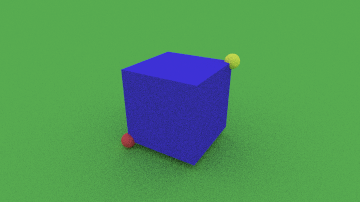
\includegraphics[width=.7\textwidth]{imgs/box-vertices.png}
  \caption{Cubo azul con los 2 vértices que lo definen}
  \label{fig:box-vertices}
\end{figure}

Sobre cada uno de estos vértices ubicamos 3 planos con normales sobre cada eje,
con dirección opuesta al otro vértice, de forma que los 6 planos encapsulen el
volumen del cubo.

Debido a que los planos son infinitos y están sobre cada eje del espacio,
cualquier rayo interseca con al menos 2 planos del cubo. Para decidir si alguna
de estas intersecciones corresponde a alguna cara del cubo, tenemos que
verificar que el punto se encuentre dentro del volumen del mismo (o al menos lo
suficientemente cerca). Para esto usamos las coordenadas de los 2 vértices que
definen al cubo: cada coordenada del punto de intersección debe estar entre las
coordenadas correspondientes de los vértices. Es decir, si $P_{min}=(p_1, p_2,
  p_3)$ y $P_{max}=(q_1, q_2, q_3)$ son los vértices del cubo, y $Q=(x, y, z)$ es
el punto donde el rayo interseca a una cara, el punto pertenece al cubo si:

\begin{align*}
  P_{min} \le Q \le P_{max} \iff & p_1 \le x \le q_1 \land \\
                                 & p_2 \le y \le q_2 \land \\
                                 & p_3 \le z \le q_3
\end{align*}

Como $Q$ resulta de la intersección con un plano, y el resultado no siempre es
exacto, usamos $\epsilon = 10^{-4}$ para extender el rango de valores aceptables
para $Q$ ($p_i - \epsilon \le (Q)_i \le q_i + \epsilon$).

\begin{algorithm}
  \begin{algorithmic}[1]
    \Function{CubeHit}{$Cube, Ray, t_{min}, t_{max}$}{$\rightarrow (hit, record)$}
    \State $vmin \gets Cube.vmin$ \Comment{Obtenemos los vertices del cubo}
    \State $vmax \gets Cube.vmax$
    \State $faces \gets Cube.faces$

    \State $hitAnyFace \gets$ False
    \State $closestSoFar \gets \infty$
    \State $cubeRecord \gets$ NIL

    \For {$face \in faces$} \Comment{Cada cara es un plano}
    \State {$(faceHit, faceRecord) \gets$ PlaneHit($face, Ray, t_{min}, closestSoFar$)}
    \State {$insideBox \gets$ puntoEntreVertices($faceRecord.p, vmin, vmax$)}

    \If {$faceHit \land insideBox$}
    \State {$hitAnyFace \gets$ True}
    \State {$closestSoFar \gets faceRecord.t$}
    \State {$cubeRecord \gets faceRecord$}
    \EndIf
    \EndFor

    \State \Return ($hitAnyFace, cubeRecord$)
    \EndFunction
  \end{algorithmic}
  \caption{Algoritmo \textit{hit} para cubos}
  \label{alg:box-hit}
\end{algorithm}

En el algoritmo \ref{alg:box-hit}, $hitAnyFace$ es \texttt{True} si y solo si el
rayo $Ray$ interseca a alguna cara del cubo y lo hace dentro de las coordenadas
definidas por los límites del mismo ($vmin$ y $vmax$). En ese caso, se actualiza
$closestSoFar$ para ignorar las próximas intersecciones que podrían quedar detrás
de la más cercana a la cámara, y se guarda el registro de la intersección en
$cubeRecord$.

\subsubsection{Triángulos}

Nuevamente, podemos utilizar lo que conocemos sobre planos para definir un
triángulo. Al definir el triángulo con 3 puntos, definimos también el plano sobre
el que se encuentra. Para acomodarnos a la representación que adoptamos para los
planos, podemos usar alguno de los vértices como origen, y calcular la normal
como el producto vectorial de los vectores que salen del origen a los otros 2
vértices (ver figura \ref{fig:triangle-normal}).

\begin{figure}
    \centering
    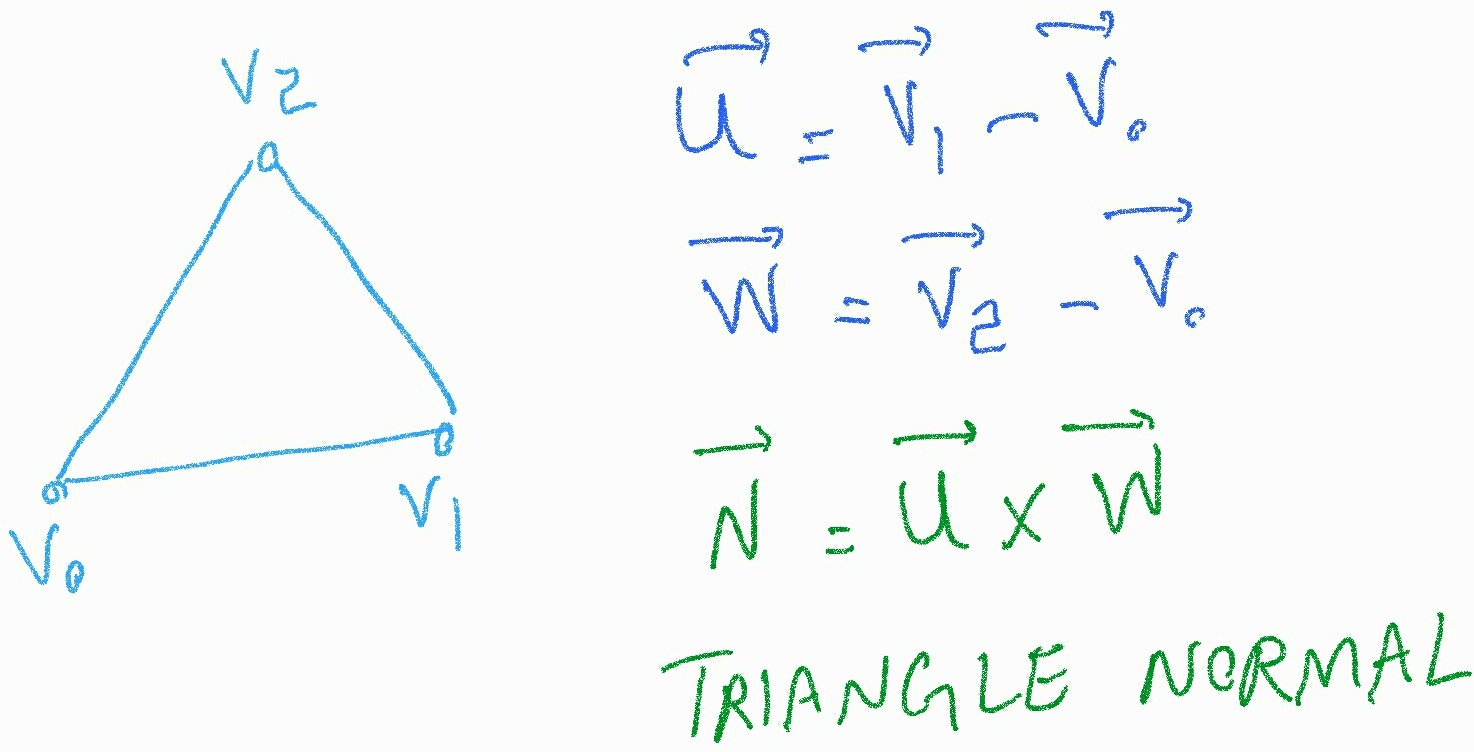
\includegraphics[width=.7\textwidth]{imgs/triangle-normal.jpg}
    \caption{Vertices de un triángulo y la normal al plano}
    \label{fig:triangle-normal}
\end{figure}

Al igual que hicimos con el cubo, primero calcularemos el punto de intersección
entre el rayo y el plano, y luego verificaremos que el punto se encuentre entre
los vértices del triángulo para determinar si el rayo interseca o no con el
mismo. Para verificar esto, tenemos que definir una convención para indicar que
cara del triángulo es la ``visible'' (es decir, en que sentido apunta la normal
del plano). Diremos que el lado visible es el que se muestra en la figura
\ref{fig:triangle-normal}, es decir, el lado en el que los vértices $v_0$, $v_1$
y $v_2$ aparecen en sentido anti-horario.

Si sabemos que los vértices aparecen en cierto orden, detectar un punto dentro
de la superficie del triangulo consiste en verificar que el punto se encuentra
``dentro'' para cada borde. Es decir, sea $P$ un punto en el plano de
intersección, sí:

\begin{itemize}
  \item $(v_2 - v_1) \times (P - v_1)$ apunta en el sentido de la normal,
  \item $(v_3 - v_2) \times (P - v_2)$ apunta en el sentido de la normal, y
  \item $(v_1 - v_3) \times (P - v_3)$ apunta en el sentido de la normal
\end{itemize}

, significa que $P$ esta ``dentro'' del triángulo para cada borde. Luego,
determinar si 2 vectores sobre la misma dirección apuntan hacia el mismo sentido
es tan fácil como ver que su producto interno es positivo. El algoritmo
\ref{alg:triangle-hit} sigue estos pasos para determinar la intersección.

\begin{algorithm}
  \begin{algorithmic}[1]
    \Function{TriangleHit}{$Triangle, Ray, t_{min}, t_{max}$}{$\rightarrow (hit, record)$}
    \State $P_1, P_2, P_3 \gets Triangle$ \Comment{Obtenemos los vertices del triangulo}
    \State $normal \gets (P_2 - P_1) \times (P_3 - P_1)$

    \If {$normal \perp Ray.dir$}
    \State \Return (False, NIL) \Comment{Si el rayo es paralelo al plano, no hay hit}
    \EndIf

    \State $t \gets ((P_1 - Ray.origin) \cdot normal) / (Ray.dir \cdot normal)$
    \If {$\lnot (t_{min} \le t \le t_{max})$}
    \State \Return (False, NIL)
    \EndIf

    \State $P \gets Ray.at(t)$ \Comment{Punto de intersección}
    \State $dentroBorde1 \gets normal \cdot ((P_2 - P_1) \times (P - P_1)) > 0$
    \State $dentroBorde2 \gets normal \cdot ((P_3 - P_2) \times (P - P_2)) > 0$
    \State $dentroBorde3 \gets normal \cdot ((P_1 - P_3) \times (P - P_3)) > 0$


    \If {$dentroBorde1 \land dentroBorde2 \land dentroBorde3$}
    \State $record \gets (t, p, normal, \dots)$
    \State \Return (True, $record$)
    \EndIf

    \State \Return (False, NIL)
    \EndFunction
  \end{algorithmic}
  \caption{Algoritmo \textit{hit} para triángulos}
  \label{alg:triangle-hit}
\end{algorithm}

\subsubsection{KDTree}

El KDTree es una estructura que agrupa muchos objetos y optimiza la búsqueda del
objeto con el que finalmente intersecan los rayos.

Consiste de una jerarquía de nodos que forman un árbol binario, en el que cada
uno o bien tiene una lista de objetos (nodo hoja), o bien tiene dos nodos hijos
(nodo intermedio). Cada nodo es representado por un \textbf{cubo} llamado
\textit{bounding box}, que está definido como:

\begin{itemize}
  \item Para nodos hoja: el cubo más chico que contiene a todos los objetos en su interior
  \item Para nodos intermedios: el cubo más chico que contiene a los cubos de
        sus nodos hijos.
\end{itemize}

Para crear un KDTree, se necesita un conjunto de objetos que contendrá la
estructura, y una cantidad \textit{max leaf size}. Luego, se crea un nodo que
contenga a todos los objetos, y se lo ``divide'' en dos nodos hijos mientras
cada nodo tenga más de \textit{max leaf size} objetos. Los objetos del nodo
padre se dividen en dos mitades (usando el eje sobre el que están mejor
distribuidos como referencia), y se reparten a cada nodo hijo.

\begin{figure}[H]
  \centering
  \begin{subfigure}[b]{0.45\textwidth}
    \centering
    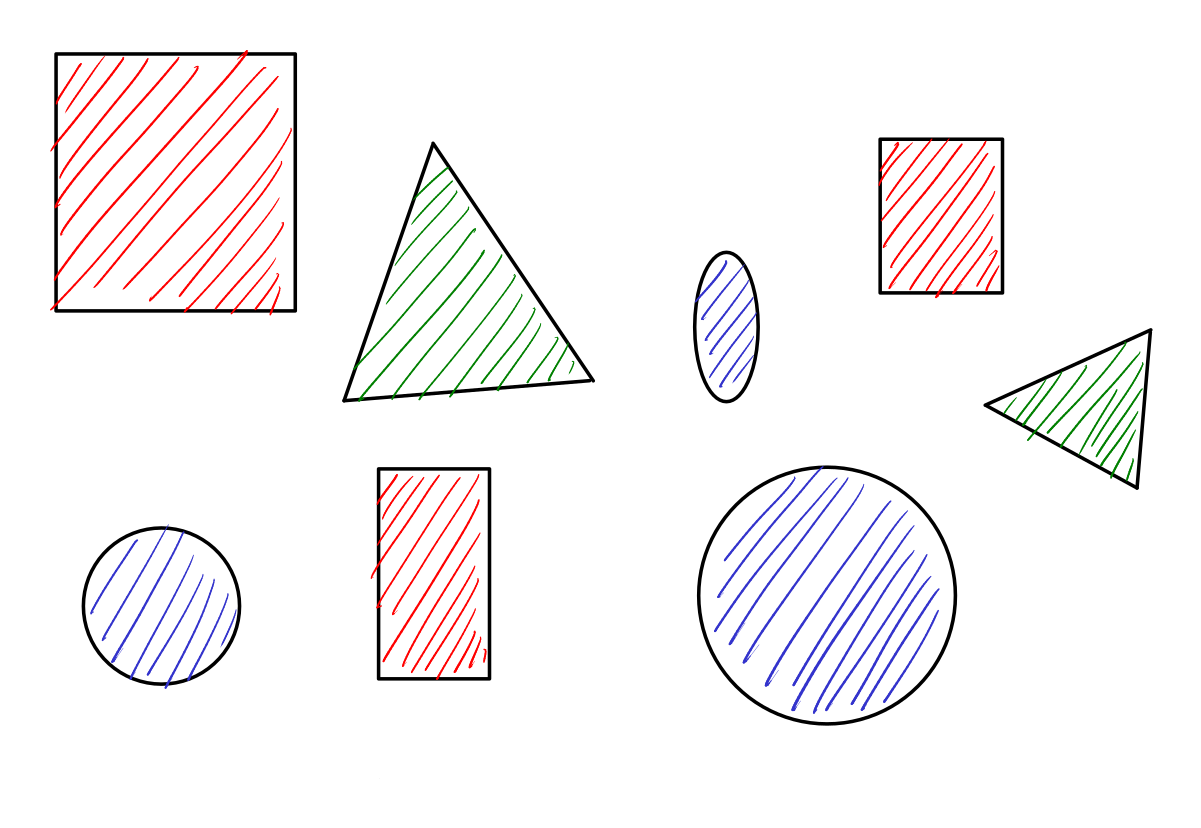
\includegraphics[width=\textwidth]{imgs/kdtree-scene-without-bbox.png}
    \caption{Sin \textit{bounding boxes}.}
    \label{fig:kdtree-without-bounding-boxes}
  \end{subfigure}
  \hfill
  \begin{subfigure}[b]{0.45\textwidth}
    \centering
    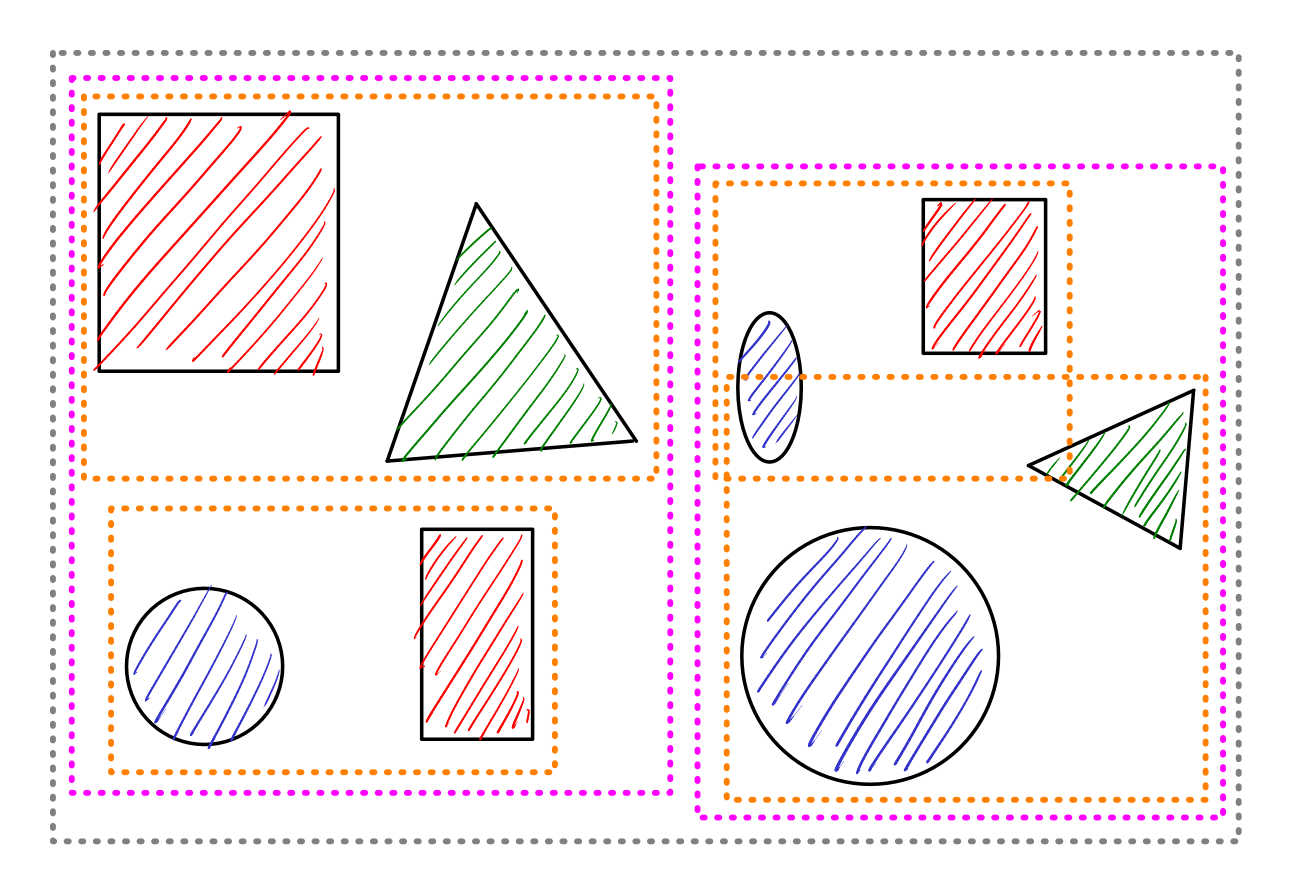
\includegraphics[width=\textwidth]{imgs/kdtree-scene-with-bbox.png}
    \caption{Con \textit{bounding boxes}: en gris del nodo raíz, en rosa
      nodos del primer nivel, y naranja del segundo.}
    \label{fig:kdtree-with-bounding-boxes}
  \end{subfigure}
  \caption{Escena 2D con y sin \textit{bounding boxes} para un \textit{max
      leaf size} de 2.}
  \label{fig:kdtree-bounding-boxes}
\end{figure}

En la figura \ref{fig:kdtree-bounding-boxes} podemos observar como se
distribuyen los \textit{bounding boxes} de cada nodo del KDTree. El nodo raíz
contiene a todos los objetos, los nodos del primer nivel del árbol se
reparten los objetos a la mitad usando el eje horizontal como referencia (en
rosa), y finalmente los del segundo nivel los reparten usando eje vertical (en
naranja).

El KDTree optimiza el cálculo de intersección de rayos con sus objetos
utilizando los \textit{bounding boxes}. En lugar de calcular la intersección
entre un rayo y cada objeto, hacemos una búsqueda binaria en la jerarquía de
nodos, intersecando el rayo con el \textit{bounding box} de cada nodo.

\begin{figure}[H]
  \centering
  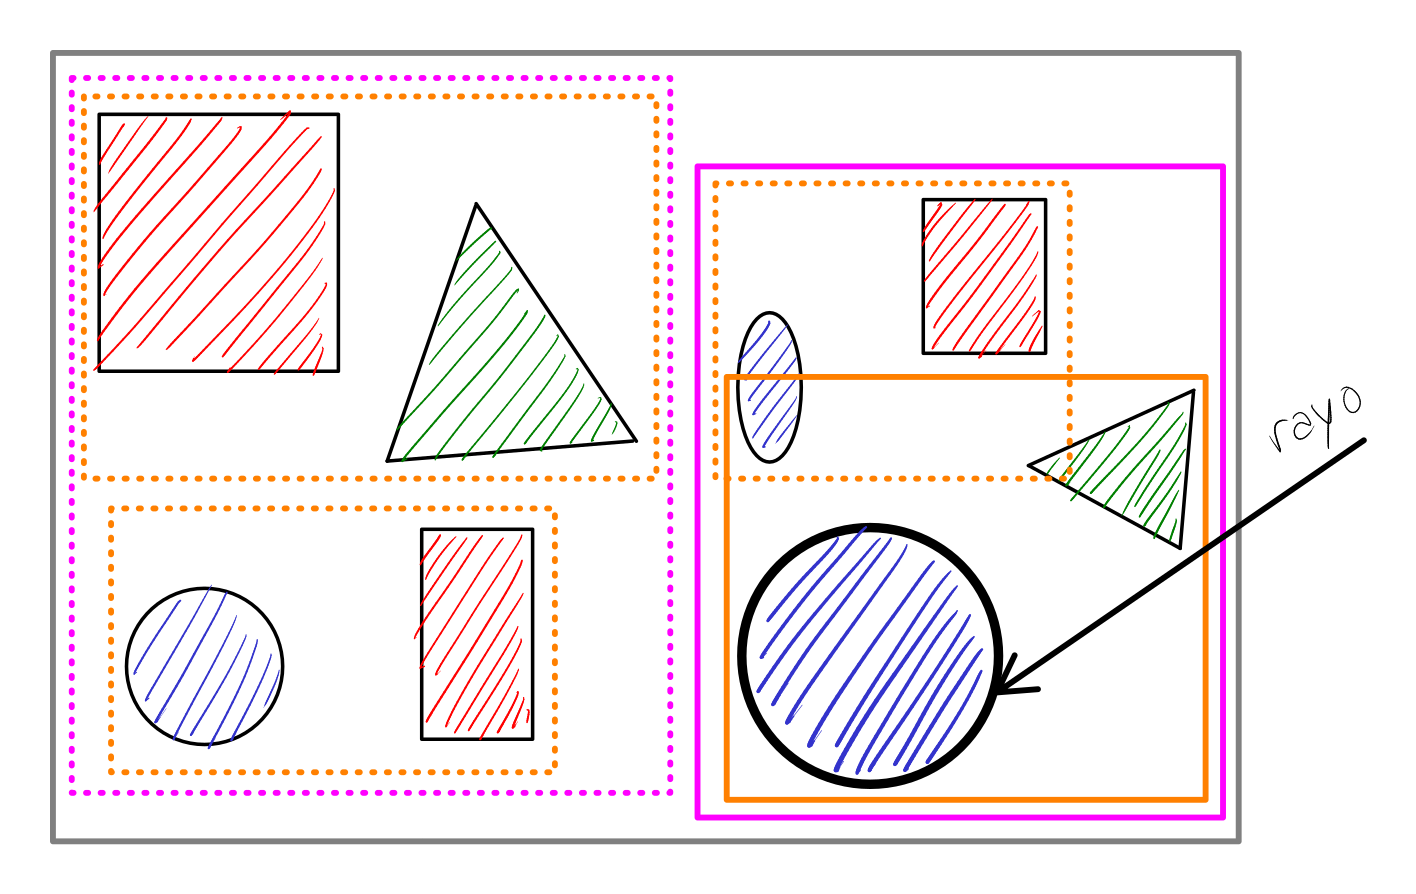
\includegraphics[width=\textwidth]{imgs/kdtree-ray-intersection.png}
  \caption{Intersección entre un rayo y el KDTree}
  \label{fig:kdtree-ray-intersection}
\end{figure}

Supongamos que tenemos que calcular la intersección con un rayo como se muestra
en la figura \ref{fig:kdtree-ray-intersection}. Primero calculamos la
intersección con el bounding box del nodo raíz del arbol: si no hay
intersección, tampoco la habrá con ningún objeto del KDTree. En este caso, hay
intersección, por lo que seguimos probando con los nodos hijos del nodo raíz
(borde rosa). Continuamos de la misma forma hasta llegar a un nodo que no tenga
hijos, y entonces hacemos una búsqueda lineal con los objetos que éste contiene.

Si establecemos una cantidad fija para \textit{max leaf size}, podemos optimizar
la búsqueda del objeto con el que un rayo intersecta. Por ejemplo, si tenemos un
modelo hecho en malla de triángulos (que puede tener miles de triángulos), y lo
ubicamos en una escena, usar un KDTree puede mejorar significativamente la
performance del Ray Tracer.

Si el modelo no ocupa mucho espacio de la imagen final, por cada rayo que no
intersecta con el modelo nos ahorramos miles de cálculos de intersecciones con
los triángulos de la malla, ya que simplemente se comprueba la intersección con
el bounding box del nodo raíz.

En el mejor caso (o el caso más común), la cantidad de intersecciones que se
calculan es como máximo $O(\log n)$ siendo $n$ la cantidad de triángulos. Se
puede dar un peor caso si todos los objetos están alineados sobre un eje de cara
a la cámara, de modo que los rayos intersecten a todos los objetos, por lo que
se realizarían $O(n+\log n)=O(n)$ intersecciones. Pero en mallas de triángulos
(que es el principal uso que le daremos), ese caso no es tan común.

\begin{algorithm}
  \begin{algorithmic}[1]
    \Function{NodeHit}{$Node, Ray, t_{min}, t_{max}$}{$\rightarrow (hit, record)$}
    \If {$Ray$ doesn't hit $Node.bounding\_box$}
    \State \Return (False, NIL)
    \EndIf

    \If {$Node$ is Leaf}
    \State \Return \textsc{ListHit}($Node.objects$, $Ray$, $t_{min}$, $t_{max}$)
    \Else
    \State $LeftNode \gets Node.left\_child$
    \State $RightNode \gets Node.right\_child$
    \State $LeftHit, LeftRec \gets$ \textsc{NodeHit}($LeftNode$, $Ray$,
    $t_{min}$, $t_{max}$)
    \State $RightHit, RightRec \gets$ \textsc{NodeHit}($RightNode$, $Ray$,
    $t_{min}$, $t_{max}$)

    \State $ClosestRec \gets$ NIL

    \If {$LeftHit \land RightHit$}
    \State $ClosestRec \gets closest(LeftRec, RightRec)$
    \ElsIf {$LeftHit$}
    \State $ClosestRec \gets LeftRec$
    \ElsIf {$RightHit$}
    \State $ClosestRec \gets RightRec$
    \EndIf

    \State \Return ($LeftHit \lor RightHit$, $ClosestRec$)
    \EndIf
    \EndFunction
  \end{algorithmic}
  \caption{Algoritmo \textit{hit} para nodos de un KDTree}
  \label{alg:node-hit}
\end{algorithm}

La implementación del KDTree en el algoritmo \ref{alg:node-hit} no hace más que
recorrer los nodos del árbol desde el nodo raíz hacia las hojas que contienen la
lista de objetos. Como ya mencionamos, se puede dar que para un nodo ambos
hijos devuelvan una intersección. Lo que se hace en ese caso es explorar ambas
ramas del árbol hasta llegar a los objetos en cuestión, y devolver la
intersección que sea más cercana a la cámara (es decir, la que finalmente se
puede ver).

El método \textsc{ListHit} que aparece en el algoritmo simplemente hace una
búsqueda lineal en una lista de objetos, y devuelve la intersección más cercana
a la cámara.

\subsection{Materiales}

Los materiales están asociados a cada objeto y se encargan de darle color a una
escena. Cada material puede emitir / atenuar luz y reflejar / refractar
rayos. En este trabajo, se implementaron 4 tipos:

\begin{itemize}
  \item Luz Difusa
  \item Lambertiano
  \item Metal
  \item Dieléctrico
\end{itemize}

Cada material implementa 2 métodos: \texttt{Scatter} (atenuar / dispersar) y
\texttt{Emit} (emitir):

\begin{itemize}
  \item \texttt{Scatter} recibe 3 parámetros: el material ($M$) sobre el que
        incide el rayo, el rayo en cuestión ($R_{in}$), y la metadata de la
        colisión ($rec$) que se dio sobre el objeto al que esta asociado el
        material. Devuelve 3 valores: \texttt{did\_scatter} que indica si el
        material puede dispersar rayos en el punto de intersección,
        $R_{out}$ el rayo dispersado en caso de que el anterior sea
        \texttt{TRUE}, y $A$ la atenuación del color que produce el material.
  \item \texttt{Emit} solamente recibe el material $M$ y retorna el color que
        emite el mismo.
\end{itemize}

Estos métodos serán llamados por cada rayo que se genere desde la cámara.
\texttt{Scatter} se encarga de dirigir cada rayo en cada colisión, hasta llegar
a un material que no disperse más (\texttt{did\_scatter} en \texttt{False}), o
hasta que se supere el \texttt{max\_depth} de la imagen.

Por la naturaleza de los materiales que se eligieron, Luz Difusa solamente emite
luz, y el resto solamente atenúa luz  y refleja / refracta los rayos que
reciben. A continuación describiremos como se implementa estos métodos, y en los
casos en los que se omita alguno se toma por defecto que \texttt{Emit} devuelve
un color negro \texttt{\#000000} (es decir, no emite luz), y que
\texttt{Scatter} devuelve \texttt{(False, NIL, NIL)} (es decir, ni atenúa ni
dispersa).

\subsubsection{Luz Difusa}

Para crear este material solo necesitamos un color $A$, que será el valor que se
devuelva al llamar al método \texttt{Emit} sobre el mismo.

\begin{algorithm}
  \begin{algorithmic}[1]
    \Function{DiffuseLightEmit}{$Light$}{$\rightarrow A$}
    \State \Return $Light.A$
    \EndFunction
  \end{algorithmic}
  \caption{Algoritmo \textit{Emit} para Luz Difusa}
  \label{alg:diffuse-light-emit}
\end{algorithm}

\subsubsection{Lambertiano}

Un material difuso o lambertiano se caracteriza por verse uniformemente
iluminado de todas las direcciones. Si bien posee un color propio $A$, también
toma parte de los colores de su entorno para formar el color final de la imagen.

\begin{algorithm}
  \begin{algorithmic}[1]
    \Function{LambertianScatter}{$Lambertian, r_{in}, rec$}{$\rightarrow
        (did\_scatter, A, R_{out})$}

    \State $scatterdir \gets rec.normal +$ (vector random en esfera unitaria)

    \If {$scatterdir \approx \vec{0}$}
    \State $scatterdir \gets rec.normal$
    \EndIf

    \State $r_{out} \gets \left \langle rec.p, scatterdir \right \rangle$
    \State \Return (True, $Lambertian.A$, $r_{out}$)
    \EndFunction
  \end{algorithmic}
  \caption{Algoritmo \textit{Scatter} para material Lambertiano}
  \label{alg:lambertian-scatter}
\end{algorithm}

Para simular el aporte uniforme de todo el entorno, en el algoritmo
\ref{alg:lambertian-scatter} tomamos como referencia la normal al plano de
intersección $rec.normal$ y le sumamos un vector random $v$ en la esfera
unitaria (es decir, $v \in \mathbb{R}^3, \vert v \vert = 1$). Puede ocurrir que
$rec.normal \approx -v$, lo cual resulte en un $scatterdir \approx 0$. En ese
caso, simplemente tomamos $scatterdir = rec.normal$.

\subsubsection{Metal}

Por otro lado, los materiales metálicos están caracterizados por reflejar muy
bien los rayos, dependiendo de que tan ``pulido'' esté el mismo. Vamos a
parametrizar un material metálico nuevamente con un color $A$, y con un valor de
\textit{fuzziness} $f \in [0, 1]$. Si $f=0$, los rayos se reflejan perfectamente
sobre la superficie, mientras que para $f>0$, se le suma algo de aleatoriedad al
rayo de salida, cuyo aporte incrementa con $f$.

\begin{algorithm}
  \begin{algorithmic}[1]
    \Function{MetalScatter}{$Metal, r_{in}, rec$}{$\rightarrow
        (did\_scatter, A, R_{out})$}

    \State $d \gets r_{in}.dir$
    \State $n \gets rec.normal$
    \State $reflected \gets d - 2 (d \cdot n) n $

    \If {$reflected \cdot n \le 0$}
    \State \Return (False, NIL, NIL)
    \EndIf

    \State $scatterdir \gets reflected + Metal.f \times$ (vector random en esfera
    unitaria)

    \State $r_{out} \gets \left \langle rec.p, scatterdir \right \rangle$
    \State \Return (True, $Metal.A$, $r_{out}$)
    \EndFunction
  \end{algorithmic}
  \caption{Algoritmo \textit{Scatter} para material metálico}
  \label{alg:metal-scatter}
\end{algorithm}

Como vemos en el algoritmo \ref{alg:metal-scatter}, la aleatoriedad la provee un
vector random en la esfera unitaria. En caso de que el rayo reflejado no se
encuentre del lado de la cara de la superficie ($reflected \cdot n \le 0$), el
material no dispersa el rayo y devuelve \texttt{(False, NIL, NIL)}.

\subsubsection{Dieléctrico}

Los materiales dieléctricos son aquellos que al recibir rayos de luz, son
capaces de separarlos en un rayo que se refleja, y otro que se refracta. Si bien
nuestra representación solo permite un rayo de salida, simularemos este
comportamiento reflejando y refractando rayos en cada punto de un objeto de
manera aleatoria.

\begin{figure}
  \centering
  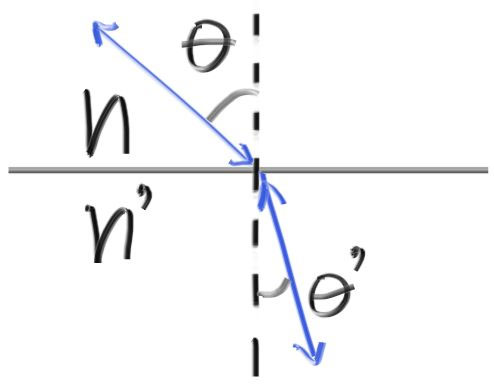
\includegraphics[width=.35\textwidth]{imgs/refraction.jpg}
  \caption{Ley de Snell}
  \label{fig:snell-law}
\end{figure}

Ya vimos como calcular el rayo reflejado, así que veremos como calcular el
refractado. Así como un rayo se refleja al entrar en contacto con una
superficie, la refracción se da en la frontera entre 2 materiales con índices de
refracción $\eta$ y $\eta'$ (ver figura \ref{fig:snell-law}). Si el rayo viaja
por un material ($\eta$), y llega a la frontera con otro material ($\eta'$), el
ángulo de ``entrada'' en el primer material $\theta$ y el ángulo de ``salida'' en el
segundo material $\theta'$ están relacionados por la ley de Snell:

\[
  \eta \sin \theta = \eta' \sin \theta'
\]

Suponiendo que conocemos $\eta$ y $\eta'$ (uno es el índice del material, y el
otro podemos asumir que es el índice del aire), y como además conocemos $\theta$
(el ángulo con el que un rayo incide sobre una superficie respecto de la
normal), podemos calcular $\sin \theta'$ despejando de la ecuación:

\[
  \sin \theta' = \frac{\eta}{\eta'} \sin \theta
\]

El rayo refractado que se encuentra del otro lado de la frontera es $R'$, y se
puede descomponer en $R'_{\perp}$ perpendicular a la normal, y
$R_{\parallel}$ paralela a la normal: $R' = R'_{\perp} + R'_{\parallel}$.

Se puede probar que cada componente se calcula como:

\begin{align*}
  R'_{\perp}     & = \frac{\eta}{\eta'}(R + (-R \cdot n) n)  \\
  R'_{\parallel} & = - \sqrt{1 - \vert R'_{\perp} \vert^2} n
\end{align*}

Y finalmente, el rayo refractado se puede calcular con el algoritmo
\ref{alg:refract}.

\begin{algorithm}
  \begin{algorithmic}[1]
    \Function{Refract}{$R$, $n$, $i$}{ $\rightarrow R'$}

    \State $cos_{\theta} = \min\{-R \cdot n, 1.0\}$
    \State $R'_{\perp} = i (R + cos_{\theta} n)$
    \State $R'_{\parallel} = - \sqrt{\vert 1 - \Vert R'_{\perp} \Vert ^ 2 \vert} n$

    \State \Return $R'_{\perp} + R'_{\parallel}$
    \EndFunction
  \end{algorithmic}
  \caption{Algoritmo para refractar un rayo $R$ sobre una superficie con normal
    $n$ y relación de indices de refracción $i = \eta / \eta'$}
  \label{alg:refract}
\end{algorithm}

Si usáramos este algoritmo para definir \texttt{DielectricScatter} y calcular el
nuevo rayo, obtendríamos imágenes poco realistas, ya que los materiales
dieléctricos no siempre refractan los rayos. Por ejemplo, si el radio entre los
indices de refracción es mayor a 1, la refracción no es posible:

\[
  \sin \theta' = \frac{\eta}{\eta'} \cdot \sin \theta = i \cdot \sin \theta
\]

Como $\sin \theta' \in [0, 1]$, si $i \cdot \sin \theta > 1$, entonces no existe valor
de $\theta'$ que satisfaga la ecuación.

Además, los materiales dieléctricos son capaces de reflejar dependiendo del
ángulo sobre el que incide el rayo. Si bien existe una ecuación para determinar
ésto, podemos usar la aproximación de Schlick \cite{schlicksapprox} como una
alternativa simple y que para nuestro caso de uso alcanza. La misma se basa en
el uso de una propiedad llamada \textit{reflectance} que se calcula usando el
coseno del ángulo de incidencia y la relación entre los índices de refracción.

\begin{algorithm}
  \begin{algorithmic}[1]
    \Function{Reflectance}{$\cos_{\theta}$, $i$}{ $\rightarrow R'$}
    \State $r \gets \frac{1 - i}{1 + i}$
    \State \Return $r^2 + (1-r^2) (1 - \cos_{\theta})^5$
    \EndFunction
  \end{algorithmic}
  \caption{Calculó de la \textit{reflectance}}
  \label{alg:reflectance}
\end{algorithm}

El algoritmo \ref{alg:reflectance} calcula este valor. Lo que luego se pide en
la aproximación es que sea mayor que un valor aleatorio entre $[0, 1]$.

\begin{algorithm}
  \begin{algorithmic}[1]
    \Function{DielectricScatter}{$Dielectric, r_{in}, rec$}{$\rightarrow
        (did\_scatter, A, R_{out})$}
    \State $r \gets Dielectric.ir$
    \If {hit in $rec$ was front face}
    \State $r \gets Dielectric.ir^{-1}$
    \EndIf
    \State $u \gets normalized(r_{\text{in}}.direction)$
    \State $\cos_{\theta} \gets \min(1, -u \cdot rec.normal)$
    \State $\sin_{\theta} \gets \sqrt{1 - \cos_{\theta}^2}$

    \If {$r \sin_{\theta} > 1$ \textbf{or} reflectance($\cos_{\theta}, r$) $>$ (random in
        [0, 1])}
    \State $dir \gets$ reflect($u$, $rec.normal$)
    \Else
    \State $dir \gets$ refract($u, rec.normal, r$)
    \EndIf

    \State \Return (True, $Dielectric.albedo$, $\langle rec.point, dir \rangle$)
    \EndFunction
    \Function{reflect}{$v$, $n$}{$\rightarrow v'$}
    \State \Return $v - 2 (v \cdot n) n$
    \EndFunction
  \end{algorithmic}
  \caption{Algoritmo \textit{Scatter} para material dieléctrico}
  \label{alg:dielectric-scatter}
\end{algorithm}

Finalmente en el algoritmo \ref{alg:dielectric-scatter} juntamos todo lo visto.
Primero definimos $r$ como la relación entre los indices de refracción (que
depende de qué lado se da la colisión). Luego calculamos $\cos_{\theta}$ y
$\sin_{\theta}$, y decidimos si en esa oportunidad se refleja o se refracta el
rayo.
